
\section{Before the Transformers}


The Recurrent Neural Networks or RNN dates from 1986 based on the work of Rumelhart
\cite{Rumelhart}.
The Recurrent Neural Networks or RNN dates from 1986 based on the work of Rumelhart. These networks
are specialized to work with data that contains temporal information and therefore the results
obtained improve against other types such as FeedForward or Convolutional networks.


The main idea behind these models is the concept of Parameter Sharing. Con Parameter Sharing un
modelo puede generalizar mejor cuando la información esta contenida en diferentes partes de una
secuencia. Así, el modelo no necesita aprender independientemente todas las reglas que forman la
secuencias, sino que ahora, la salida para cada elemento en el tiempo esta determinada por la
salida del elemento anterior. Resultando en una recurrencia con las mismas reglas de actualización
aplicadas a cada elemento en el tiempo. La ecuación \ref{eq:rnn} representa este proceso; $h^{(t)}$
es el estado de la recurrencia aplicada por alguna función $f$ a un elemento $x^{(t)}t$ de la
secuencia $x$ en el tiempo $t$, $\theta$ son los parámetros compartidos.

\begin{equation}
    h^{(t)} = f(h^{(t-1)}, x^{(t)}; \theta)
\end{equation}
\label{eq:rnn}
\begin{figure}[]

En una RNN vista como un gráfo computacional dirigído y acíclico, cada nodo representa un estado en
la recurrencia y procesa la información de la secuencia $x$ con los mismos parámetros $\theta$ en cada
paso, observe la figura \ref{fig:rnn_cg}.

%\centering centers the figure on the page.  This is convention.
\centering

% The \includegraphics command is the default way to include a figure.  The first optional argument in [] brackets defines how large the figure should be on the page.  This can be defined in inches, centimeters, or as a fraction of the \textwidth.  Then, in the curly {} braces you will put the file name for the figure.  Here it has been stored in a subfolder entitled Figures.  You are encouraged to give your figures descriptive file names, as this will help future students to figure out what figure corresponds to which file without having to read your LaTeX code.
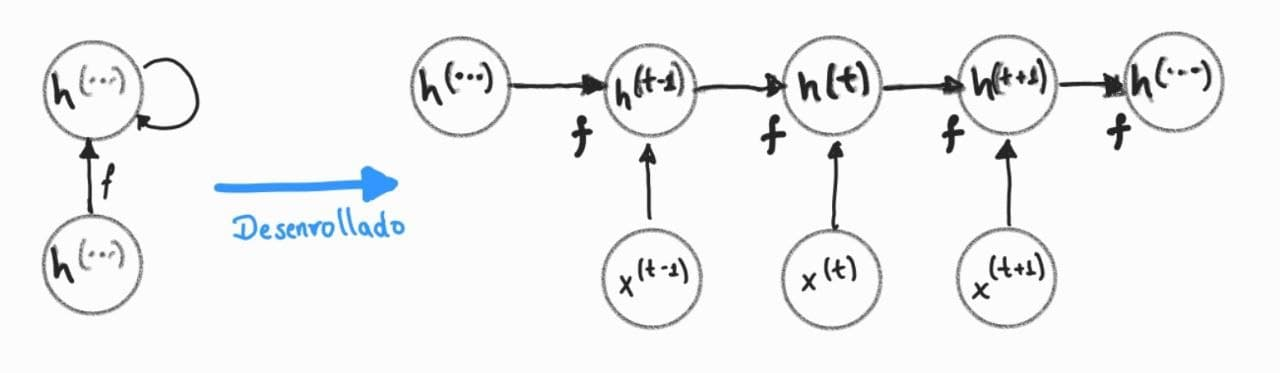
\includegraphics[width=.8\textwidth]{Chapters/1. Transformer/Figures/rnn/rnn_cgraph.jpg}

%\caption will create a figure caption.  Putting an asterisk after it (as in \caption* ) will cause the caption to not be numbered and to not appear in the list of figures.  The [] argument is optional but recommended; this is the short-form caption which will appear in the list of figures.  The {} argument is required, and gives the full caption which will appear in the main text.  The first few words of this caption will be used in the list of figures if no [] form is given.
\caption[RNN - Grafo Computacional]{Grafo computacional generado por una RNN al "desenrrollar" la
recurrencia. Usando los parámetros compartidos en cada nodo, con cada elemento $x^{(t)}$ de la
secuencia genera un nuevo estado oculto $h^{(t)}$ para retroalimentar nuevamente la entrada del
siguiente nodo.}

% the \label gives a reference for this figure so that you can refer to it in the text by its number in a way which will be automatically updated if you change the document.  THIS IS A GOOD IDEA; having automatically updated references for figures, equations, etc, will keep your document in order even as you continue to update it over a period of months.  This reference can be called in the text using the \ref tag.
\label{fig:rnn_cg}
\end{figure}
